\documentclass[12pt,fleqn]{article}
\setlength{\parindent}{0pt}
\usepackage{graphicx}
\usepackage{cancel}
\usepackage{listings}
\usepackage[latin5]{inputenc}
\usepackage{color}
\setlength{\parskip}{8pt}
\setlength{\parsep}{0pt}
\setlength{\headsep}{0pt}
\setlength{\topskip}{0pt}
\setlength{\topmargin}{0pt}
\setlength{\topsep}{0pt}
\setlength{\partopsep}{0pt}
\setlength{\mathindent}{0cm}

\begin{document}
Ders 2

Karakteristik Egriler Metodu

Bu metot katsayilari sabit olmayan 1. derece, lineer PDE cozmemize yardim
eder. PDE su formdadir

\[ \frac{\partial u}{\partial x} + 
p(x,y) \frac{\partial u}{\partial y} = 0 
\ \ \ (*)
 \]

ve $p(x,y)$, $x,y$ degiskenlerinin bir fonksiyonudur. 

Ustteki denklemi iki vektorun noktasal carpimi olarak ta gorebiliriz. 

\[ 
<\frac{\partial u}{\partial x}, \frac{\partial u}{\partial y}> \cdot 
<1,p(x,y)> = 0
 \]

Bu acidan bakinca yukaridaki ifade yeni bir sey soyluyor, $u$'nun
$<1,p(x,y)>$ vektorune gore yonsel turevinin sifir oldugunu soyluyor, yani
o yonde hicbir degisim yok. 

Simdi tek basina $<1,p(x,y)>$ vektorunu dusunelim, her degisik $x,y$ icin
bu vektorler bir vektor alani olusturur, bu alandaki vektorleri bir egrinin
``belli bir noktadaki egimini gosterdigi'' seklinde alabiliriz. O
noktalardaki egim $p(x,y) / 1$ olacaktir dogal olarak, o zaman bu egriler
icin soyle bir basit diferansiyel denklem (ODE) yazabiliriz.

\[ \frac{dy}{dx} = \frac{p(x,y)}{1} \]

ya da

\[ \frac{dy}{dx} = p(x,y) 
\ \ \ (**)
\]

Bu ODE bir yon alani (direction field) olusturur (bkz MIT OCW ODE Ders 1).

Simdi geri adim atip her seye tekrar bakalim. (*) diyor ki $x,y$ noktasinda
$u$'nun $<1,p(x,y)>$ yonundeki yonsel turevi sifir. Yani $x,y$ noktasinda
$<1,p(x,y)>$ yonunde ilerlersek $u$ hic degismeyecek. 

Ayni zamanda $<1,p(x,y)>$ vektorleri (**) icin bir yonsel alan da
tanimliyor!  Bilindigi gibi (**) denklemi cozum egrileri (solution curves)
ortaya cikartir, ve ne raslanti ki (!) bu cozum egrilerinin her birinde
(*)'deki $u$ sabit kalir. 

Ornek 

\[ \frac{\partial u}{\partial x} + 
x \frac{\partial u}{\partial y} = 0 
 \]

Yani $p(x,y) = x$. O zaman 

\[ \frac{dy}{dx} = x \]

denklemini cozeriz, ve 

\[ y = \frac{1}{2}x^2 + C \]

karakteristik egrilerini elde ederiz. Tekrar duzenlersek

\[ y - \frac{1}{2}x^2 = C \]

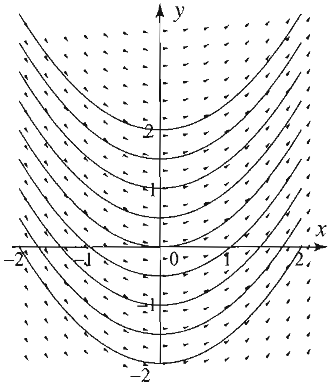
\includegraphics[height=4cm]{2_1.png}
















\end{document}
